\documentclass[12pt,a4paper]{article}
\usepackage{graphicx}
\usepackage[showframe=false]{geometry}
\usepackage{changepage}
\usepackage{floatrow}
\usepackage[colorlinks=false]{hyperref} 
\usepackage[abs]{overpic}
\usepackage{amsmath}
\usepackage{mathtools}
\usepackage{float}
\usepackage{enumitem,blindtext}
\usepackage{xcolor}
\usepackage{capt-of}
\usepackage{url}

% Default fixed font does not support bold face
\DeclareFixedFont{\ttb}{T1}{txtt}{bx}{n}{9} % for bold
\DeclareFixedFont{\ttm}{T1}{txtt}{m}{n}{9}  % for normal

% Custom colors
\usepackage{color}
\definecolor{deepblue}{rgb}{0,0,0.5}
\definecolor{deepred}{rgb}{0.6,0,0}
\definecolor{deepgreen}{rgb}{0,0.5,0}

\usepackage{listings}

% Python style for highlighting
\newcommand\pythonstyle{\lstset{
language=Python,
basicstyle=\ttm,
otherkeywords={self},             % Add keywords here
keywordstyle=\ttb\color{deepblue},
emph={MyClass,__init__},          % Custom highlighting
emphstyle=\ttb\color{deepred},    % Custom highlighting style
stringstyle=\color{deepgreen},
frame=tb,                         % Any extra options here
showstringspaces=false            % 
}}

% Python environment
\lstnewenvironment{python}[1][]
{
\pythonstyle
\lstset{#1}
}
{}

% Python for external files
\newcommand\pythonexternal[2][]{{
\pythonstyle
\lstinputlisting[#1]{#2}}}

% Python for inline
\newcommand\pythoninline[1]{{\pythonstyle\lstinline!#1!}}

\lstdefinestyle{BashInputStyle}{
  language=bash,
  basicstyle=\small\sffamily,
  %frame=tb,
  columns=fullflexible,
  backgroundcolor=\color{gray!20},
  linewidth=\linewidth,
}

\renewcommand{\UrlFont}{\small}

\begin{document}
\setlength{\parindent}{0pt}

\setlist{noitemsep}

\section{Problem}
Ilastik uses VIGRA convolution routines to compute features for the calssification process.
For large data sets, those feature computations represent the computational bottleneck in the pipeline. 
As convolutions are one of the classical applications for GPUs, they seem to be the reasonable choice for speeding up those computations. 
% - feature computation is bottleneck in classification process
% - current vigra convolution is slow
% - evaluate the improvement that comes with a GPU implementation

\section{Current situation and idea}
In the current setup, VIGRA is used via the python wrapper.
This VIGRA version/method uses only a single-thread convolution implementation.
We evaluate the performance of VIGRA gaussian filters in single-thread mode and multi-thread mode (Version 1.11) and Arrayfire gaussian filters.
% - Vigra single thread implementation
% - use a ready to use library for GPU implementation as CUDA code requires high maintenance, high effort to be efficient and flexible
% - use arrayfire

\section{Why ArrayFire?}
ArrayFire (\url{http://www.arrayfire.com}) aims to be a flexible, hardware-neutral accelerator library.
This means it is not only running on CUDA GPUs, but also includes an OpenCL backend (e.g. for AMD GPUs) and a CPU fallback.
Due to the backends for CUDA and OpenCL, it is still able to leverage many specific features, that are essential to reach high performance on GPUs (see "Why not OpenGL"). \\
Moreover, the library is under active development and it is to be expected that it will modified for new hardware in the future.
Also the ArrayFire team aims to support users as good as possible, e.g with an active user group or personal consultation. \\ \\
%+ uses CUDA and OpenCL backend
%  + makes use of many features of the respective libraries and GPUs
%+ flexible
%+ actively developed
%+ good support
%+ supports batch convolution
%- still under development, might throw some unexpected exceptions...
\textbf{Why not own CUDA code?}\\
Although CUDA implementations could improve performance by writing more hardware specific code, it would be prone to overengineering.
Also such code requires enourmous effort to make it efficient and flexible and will be a lot harder to maintain. \\ \\
% Other implementations:
% CUDA:
% + might be more 
% - high maintenance
% - a lot of effort to make it efficient 
% - danger of overengineering
\textbf{Why not OpenCV?} \\
OpenCV also provides GPU implementations.
It also seems to achieve good performance and might be a useful alternative.
Yet, we concentrated on ArrayFire.\\\\
However, there are benchmarks on ArrayFire vs OpenCV:\\
\url{http://mcclanahoochie.com/blog/2011/09/opencv-vs-libjacket-gpu-sobel-filtering/} \\
\url{http://mcclanahoochie.com/blog/2011/10/gpu-convolution-opencv-gpu-and-libjacket-part-2/} \\
\url{http://opencv-gpu.blogspot.de/} \\ \\
% %- arrayfire claims to be faster
% - OpenCV can be considered to replace VIGRA
\textbf{Why not OpenGL?} \\
OpenGL would provide a widely supported library.
As a consequence, it does not exploit all available features of specific GPUs as it is possible with CUDA or OpenCL. For example, OpenGL usually relies on texture buffers and does not make use of shared memory which is essential for fast convolutions.
Also an OpenGL implementation might result in more complicated code. \\ \\
%- does not make use of all available features of the GPUs (e.g. uses texture buffer, no shared memory)
%- might require more complicated implementation
\textbf{Why not SciPy?} \\
First test indicated that SciPy only provides a small speedup and seems to use an single-thread CPU implementation.
%SciPy
%- python tests only showed slight improvement over VIGRA
%- runs single thread in test runs

\section{Arrayfire vs VIGRA}

\subsection{Differences in border treatment (padding)}
The convolution of ArrayFire can be configured to have the same result as the VIGRA convolution, exept for one difference.
VIGRA uses reflected border padding by default, whereas ArrayFire uses zero padding at the borders.
This means ArrayFire will add zeros to the image as soon as the kernel is not overlapping entirely with the image.
Therefore results in border regions differ from default vigra results.\\
The results not affected by those differences have been tested to be equal.
%  - border treatment: AF uses 0 padding
%  - VIGRA: is more flexible
%  -> different results in border region


\subsection{Hardware used for testing}
\begin{itemize}
  \item notebook - Intel(R) Core(TM) i7-3632QM CPU @ 2.20GHz, 8 GB RAM, GeForce GT 635M (2GB), CUDA Compute 2.1
  \item littleheron - Intel(R) Xeon(R) CPU E5-2643 v3 @ 3.40GHz, 64 GB RAM, GeForce GTX TITAN X (12 GB) CUDA Compute 5.2
\end{itemize}

\subsection{C++ tests for gaussian smoothing}
\subsubsection{Total GPU time}
\begin{center}
  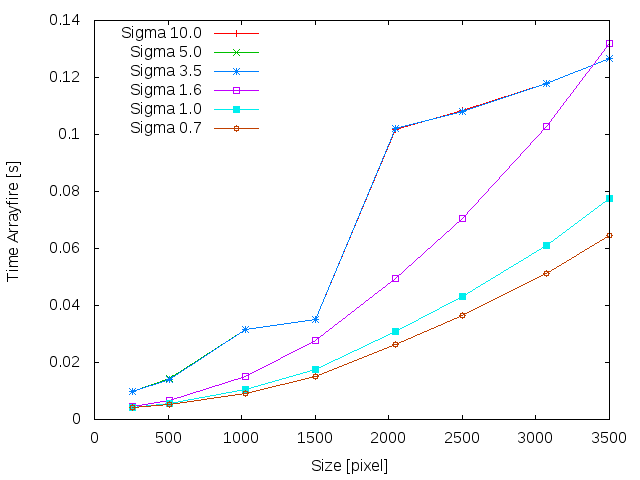
\includegraphics[width=0.8\textwidth]{media/gpu_total_notebook.png}
  \captionof{figure}{Total GPU times on notebook for different gaussian filter sizes and image sizes. Kernel size is calculated as follows: $r = \textrm{round}(3\sigma) \cdot 2 + 1$.}
\end{center}

\begin{center}
  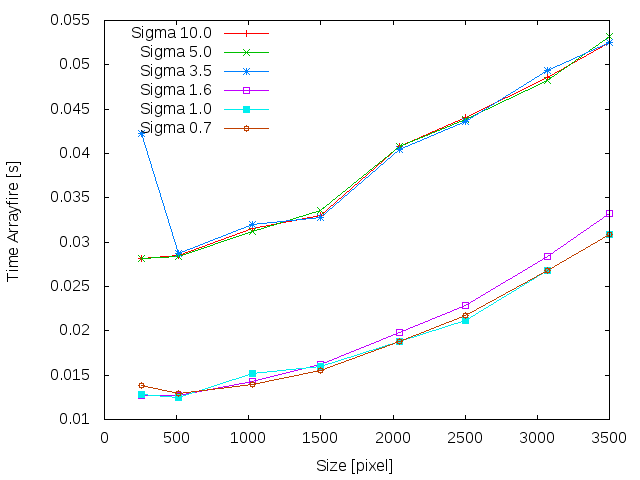
\includegraphics[width=0.8\textwidth]{media/gpu_total_littleheron.png}
  \captionof{figure}{Total GPU times on littleheron for different gaussian filter sizes and image sizes. Kernel size is calculated as follows: $r = \textrm{round}(3\sigma) \cdot 2 + 1$.}
\end{center}

\subsubsection{Ratio VIGRA single-thread vs ArrayFire}
\begin{center}
  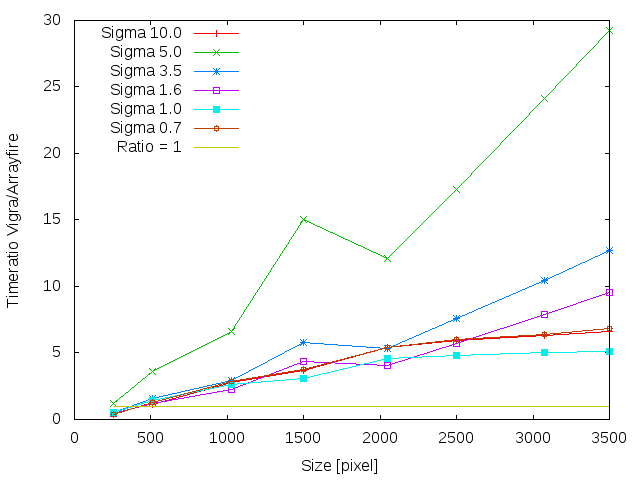
\includegraphics[width=0.8\textwidth]{media/ratio_notebook.png}
  \captionof{figure}{Ratio $\frac{\textrm{VIGRA time}}{\textrm{ArrayFire time}}$ on notebook for different gaussian filters and image sizes. We experience a speed up for ratios $> 1$.}
\end{center}

\begin{center}
  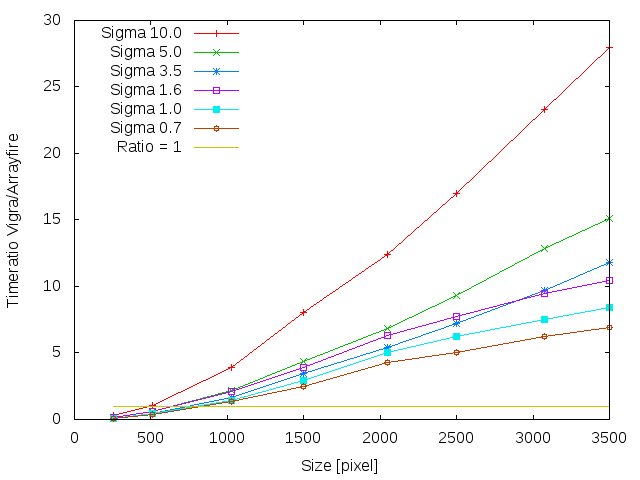
\includegraphics[width=0.8\textwidth]{media/ratio_littleheron.png}
  \captionof{figure}{Ratio $\frac{\textrm{VIGRA time}}{\textrm{ArrayFire time}}$ on littleheron for different gaussian filters and image sizes. We experience a speed up for ratios $> 1$.}
\end{center}

\subsubsection{Ratio VIGRA multi-thread vs ArrayFire}
\begin{center}
  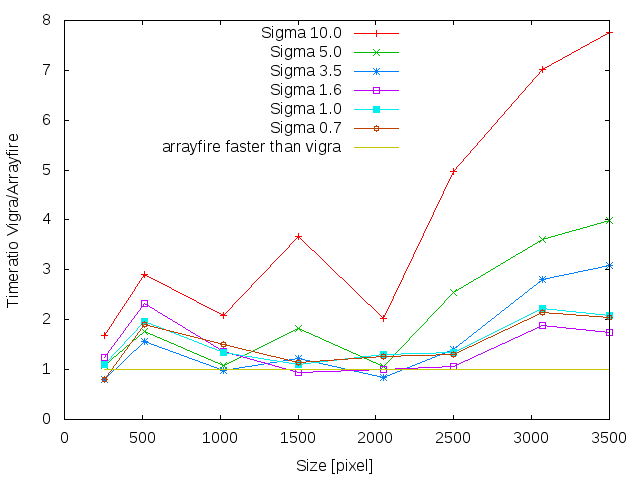
\includegraphics[width=0.8\textwidth]{media/ratio_notebook_multithread.png}
  \captionof{figure}{Ratio $\frac{\textrm{VIGRA time}}{\textrm{ArrayFire time}}$ on notebook for different gaussian filters and image sizes. We experience a speed up for ratios $> 1$.}
\end{center}

\begin{center}
  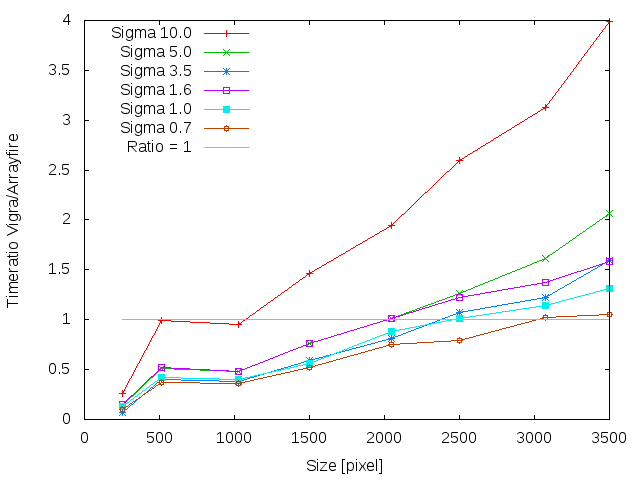
\includegraphics[width=0.8\textwidth]{media/ratio_littleheron_multithread.png}
  \captionof{figure}{Ratio $\frac{\textrm{VIGRA time}}{\textrm{ArrayFire time}}$ on littleheron for different gaussian filters and image sizes. We experience a speed up for ratios $> 1$.}
\end{center}




\end{document}
